The sensitivity of the signal regions proposed in Section~\ref{sec:sr} is evaluated with more refined statistical tools in this section, 
by using the HistFitter framework~\cite{HistFitter} to perform discovery hypothesis tests for the different signal scenarios of interest. 
The event yields assumed in these test are the ones predicted by the set of Monte-Carlo samples described in section~\ref{sec:samples}, 
and the object selections detailed in Sections~\ref{sec:objects} and~\ref{sec:evtsel}. All the results in this section are presented for an integrated luminosity of 3 fb$^{-1}$. 

The fit configuration is setup in the \textit{exclusion} mode, i.e. to perform hypothesis testing with a known BSM signal. 
Of course here the rejected hypothesis is the background-only hypothesis. 
Only one signal region is fitted at the time; furthermore, there is no control region defined in the analysis. 
We plan to investigate at a later stage potential benefits of combined fits of several signal regions, 
which was the setup in use for the Run-1 analysis. 
Distinct global systematic uncertainties are assigned to each category of background, amounting to 30\% for $t\bar t+V$ processes, $35\%$ for diboson ,100\% for minor processes such as $t\bar tH$, and 50\% for the reducible background ($t\bar t$, $V$ + jets, $W^\pm W^\mp$). 
\\
\par{\bf Event yields in the signal regions\\}

\begin{figure}[htb!]
\centering
\subfigure{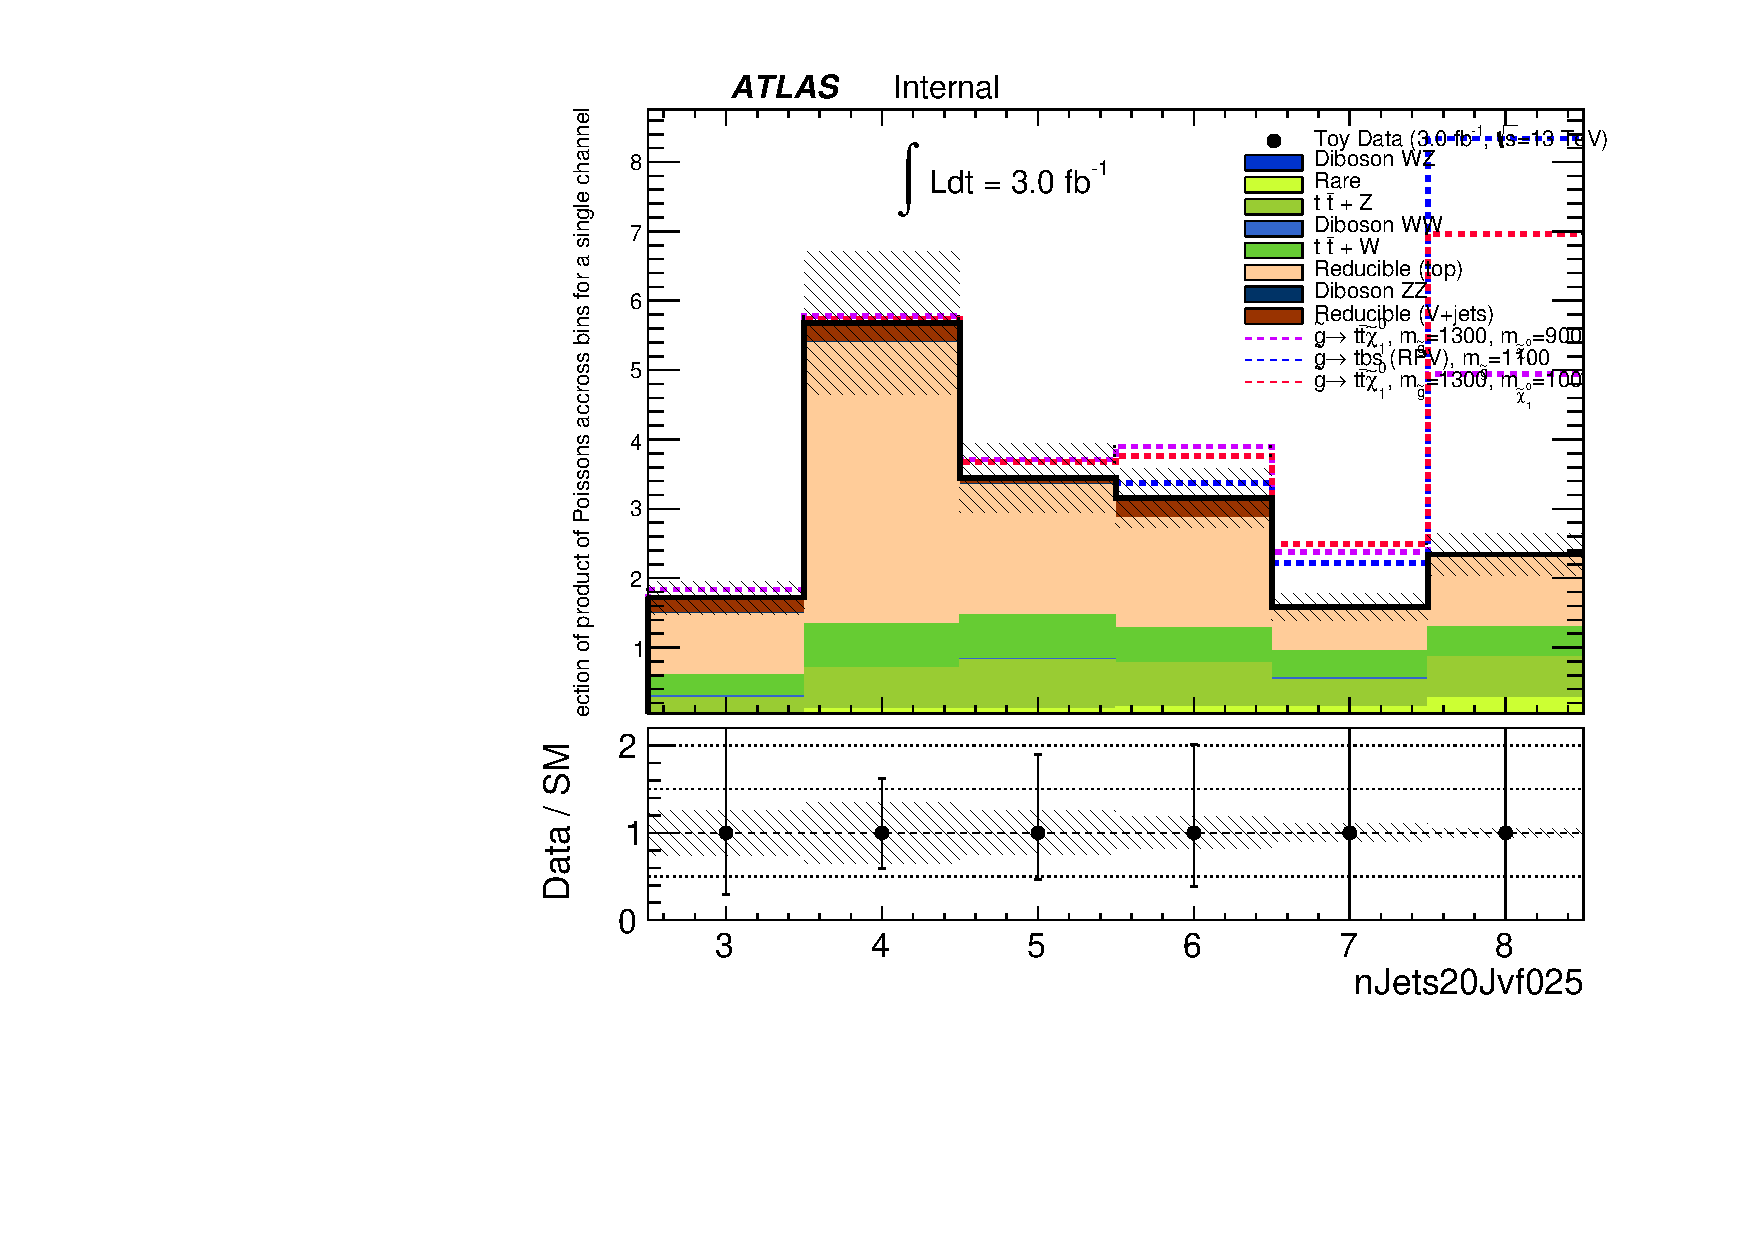
\includegraphics[width=0.49\textwidth]{HISTFITTER/can_SR3b3j20_binned_nJets20Jvf025_beforeFit}}
\subfigure{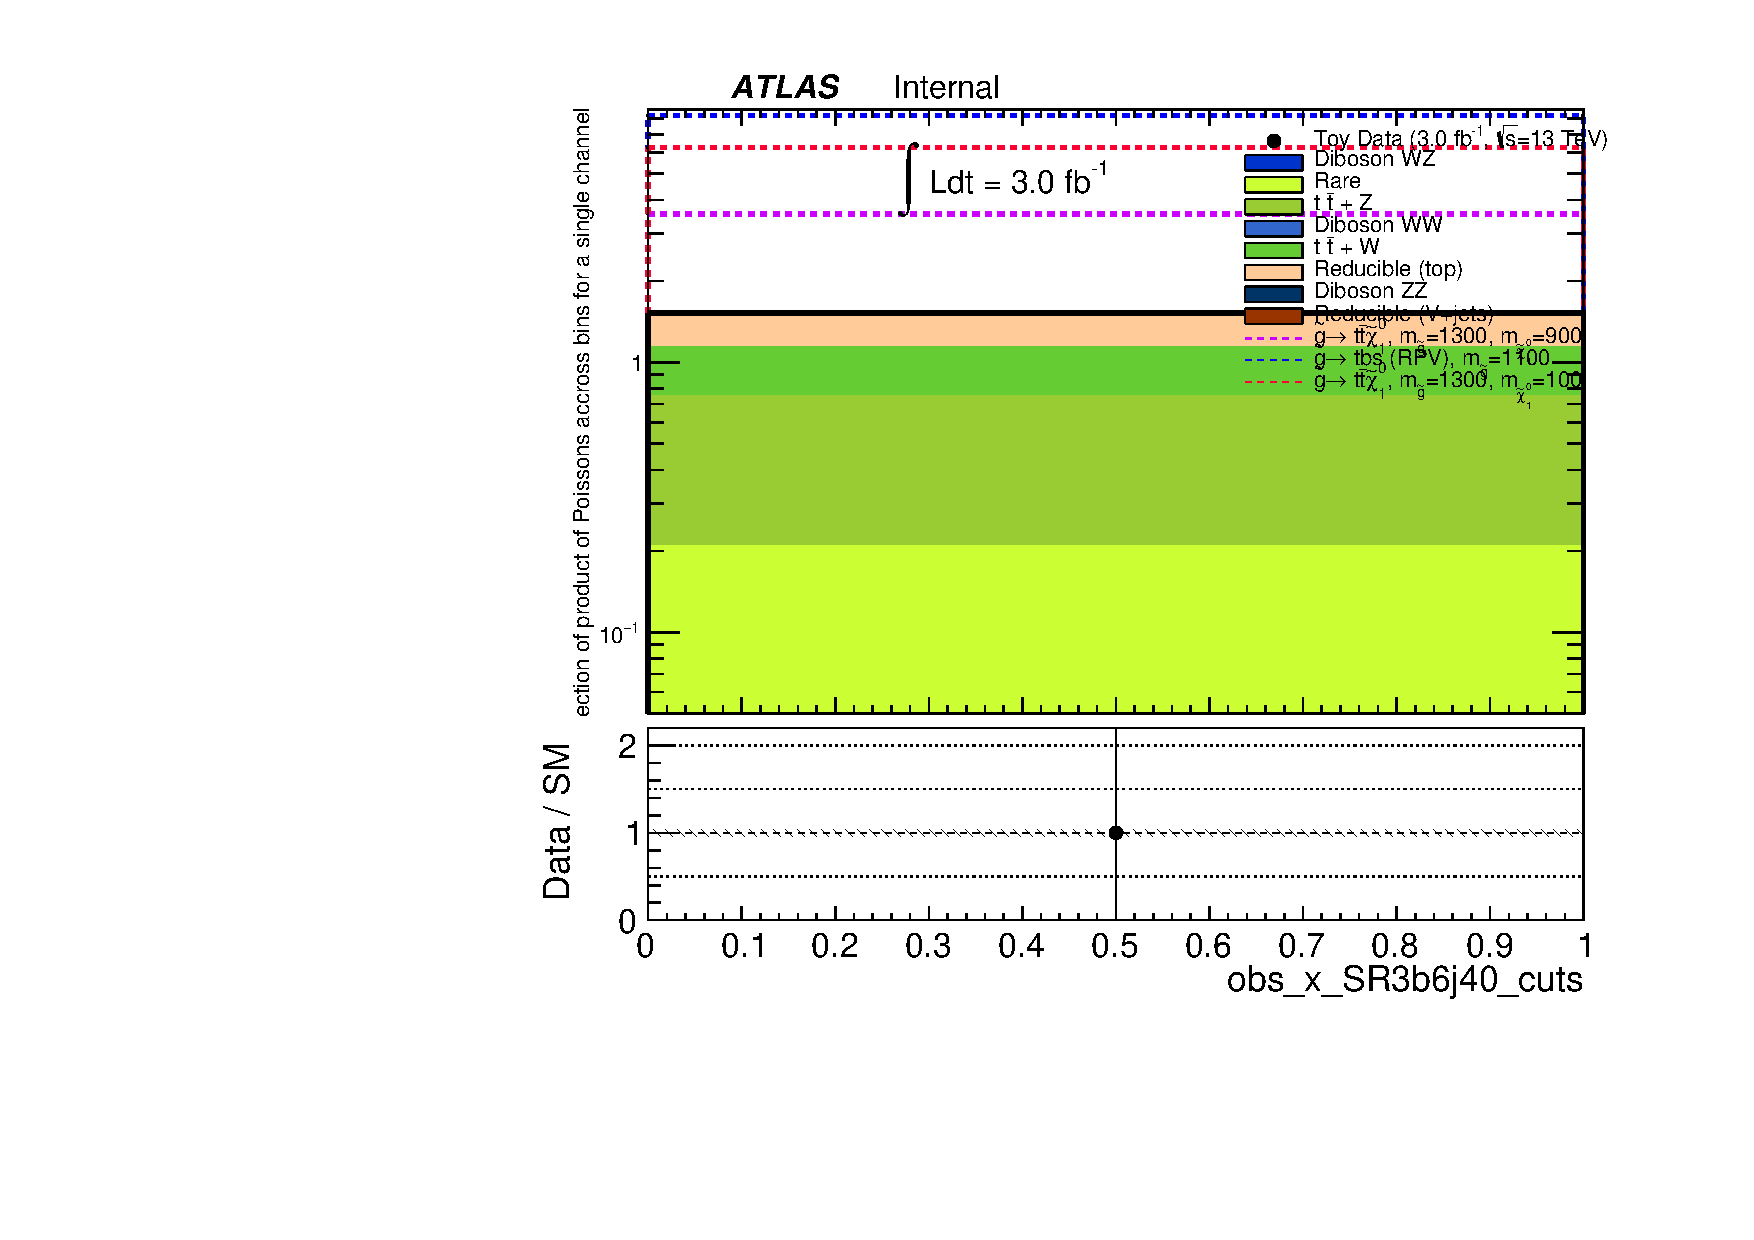
\includegraphics[width=0.49\textwidth]{HISTFITTER/can_SR3b6j40_cuts_beforeFit}}
\caption{Expected yields for Standard Model processes and a few characteristic signal scenarios, 
in selections with at least two same-sign leptons and three $b$-jets. The selection on the right side further requires at least six jets with $p_T>40$~\GeV. 
}
\label{fig:histfitter_sr3b}
\end{figure}

\begin{figure}[htb!]
\centering
\subfigure[$\met>100$, $\geq 4$ jets ($p_T>50$)]{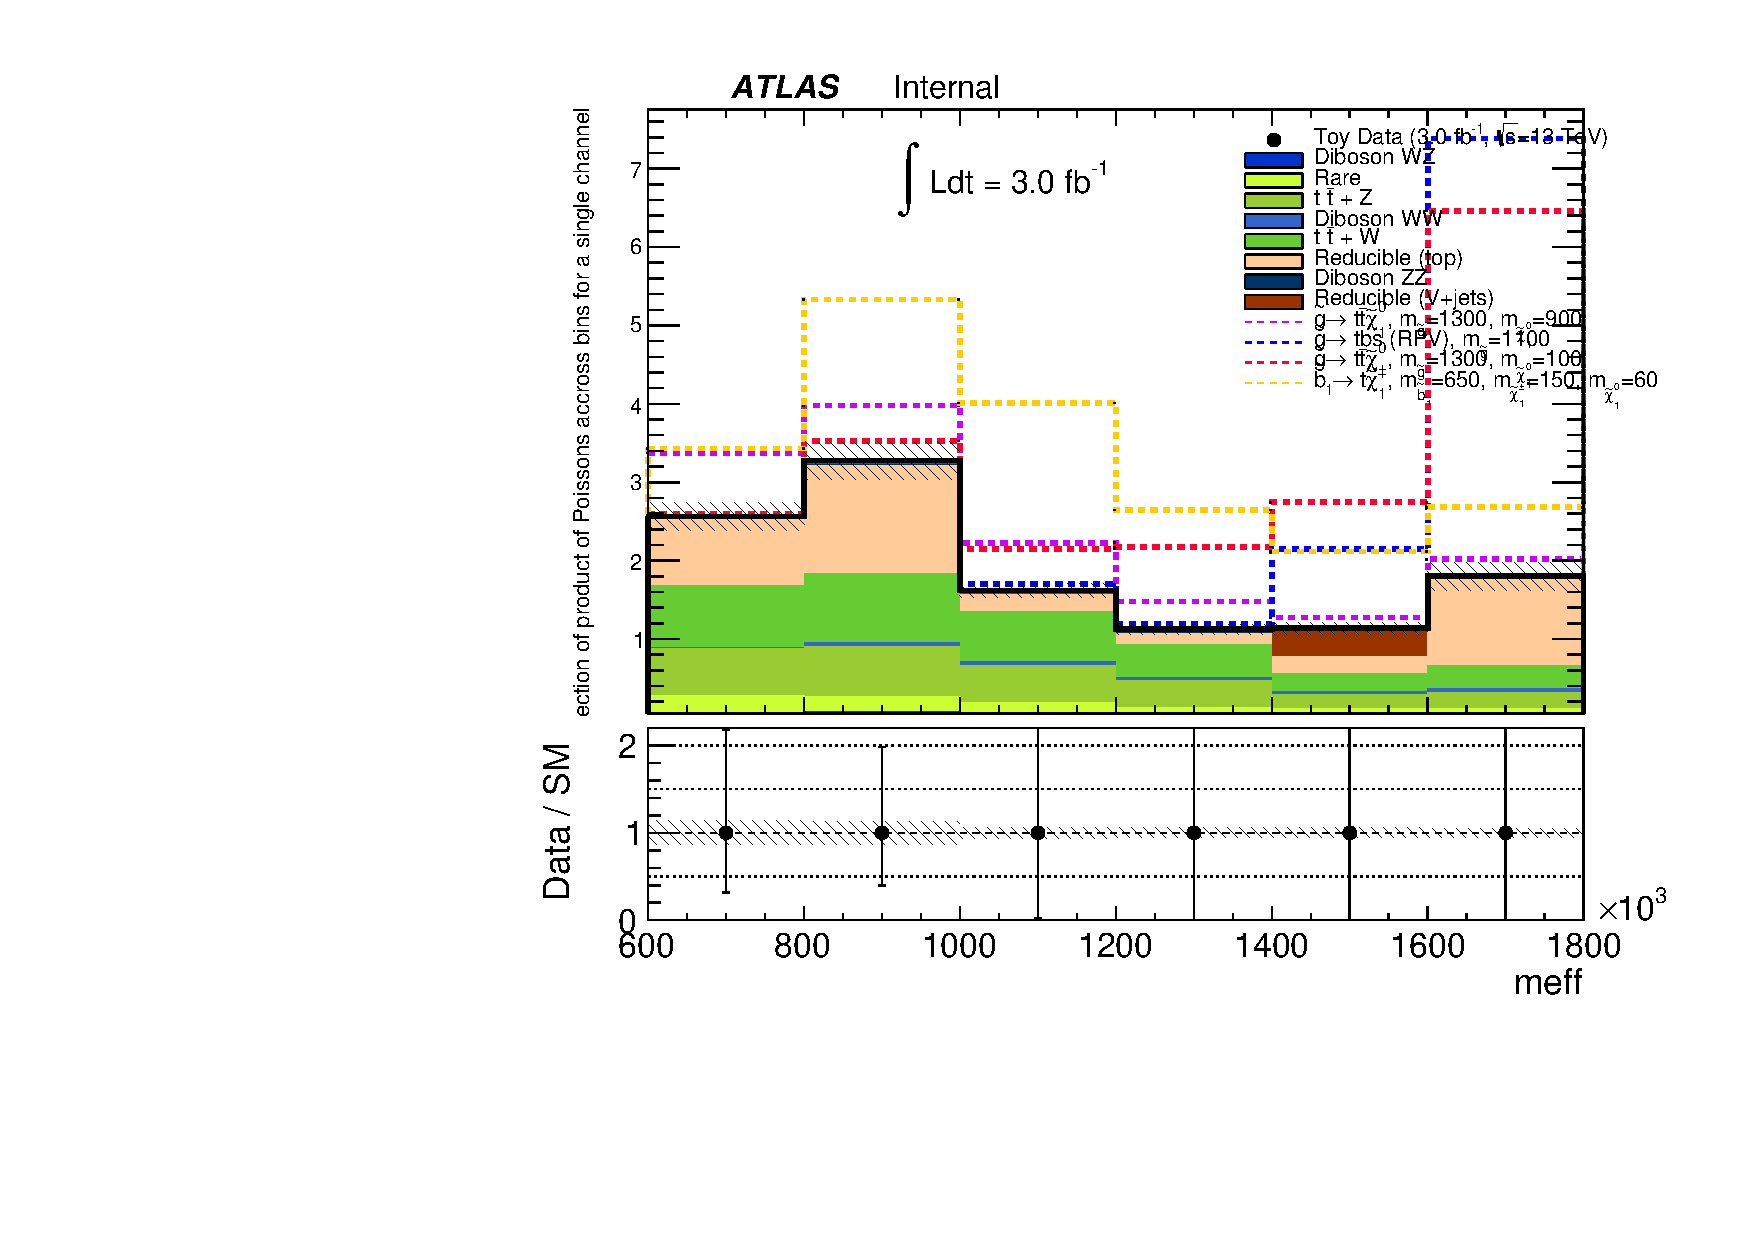
\includegraphics[width=0.49\textwidth]{HISTFITTER/can_SR1b100_binned_meff_beforeFit}}
\subfigure[$\met>100$, $\geq 3$ jets ($p_T>40$)]{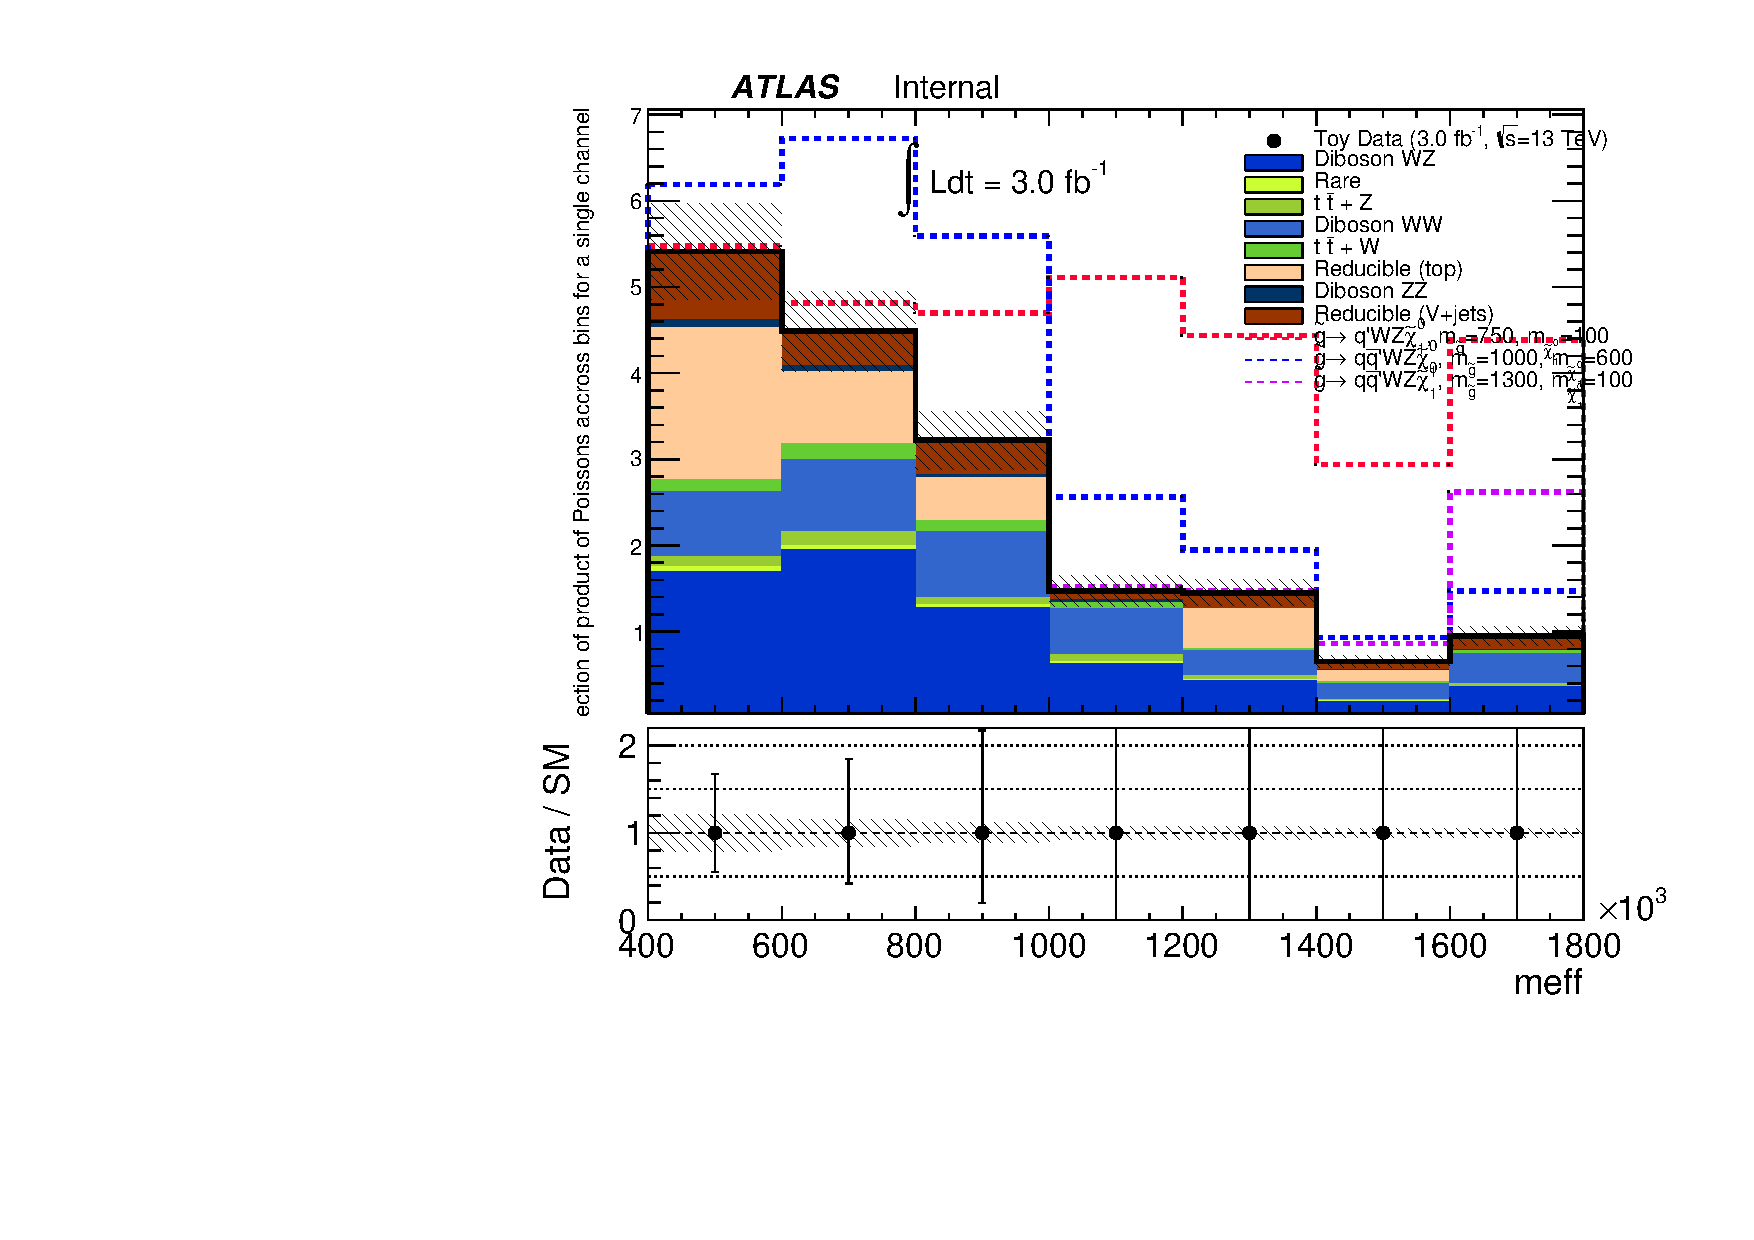
\includegraphics[width=0.49\textwidth]{HISTFITTER/can_SR0b3jmet100_binned_meff_beforeFit}}
\subfigure[$\met>150$, $\geq 4$ jets ($p_T>50$]{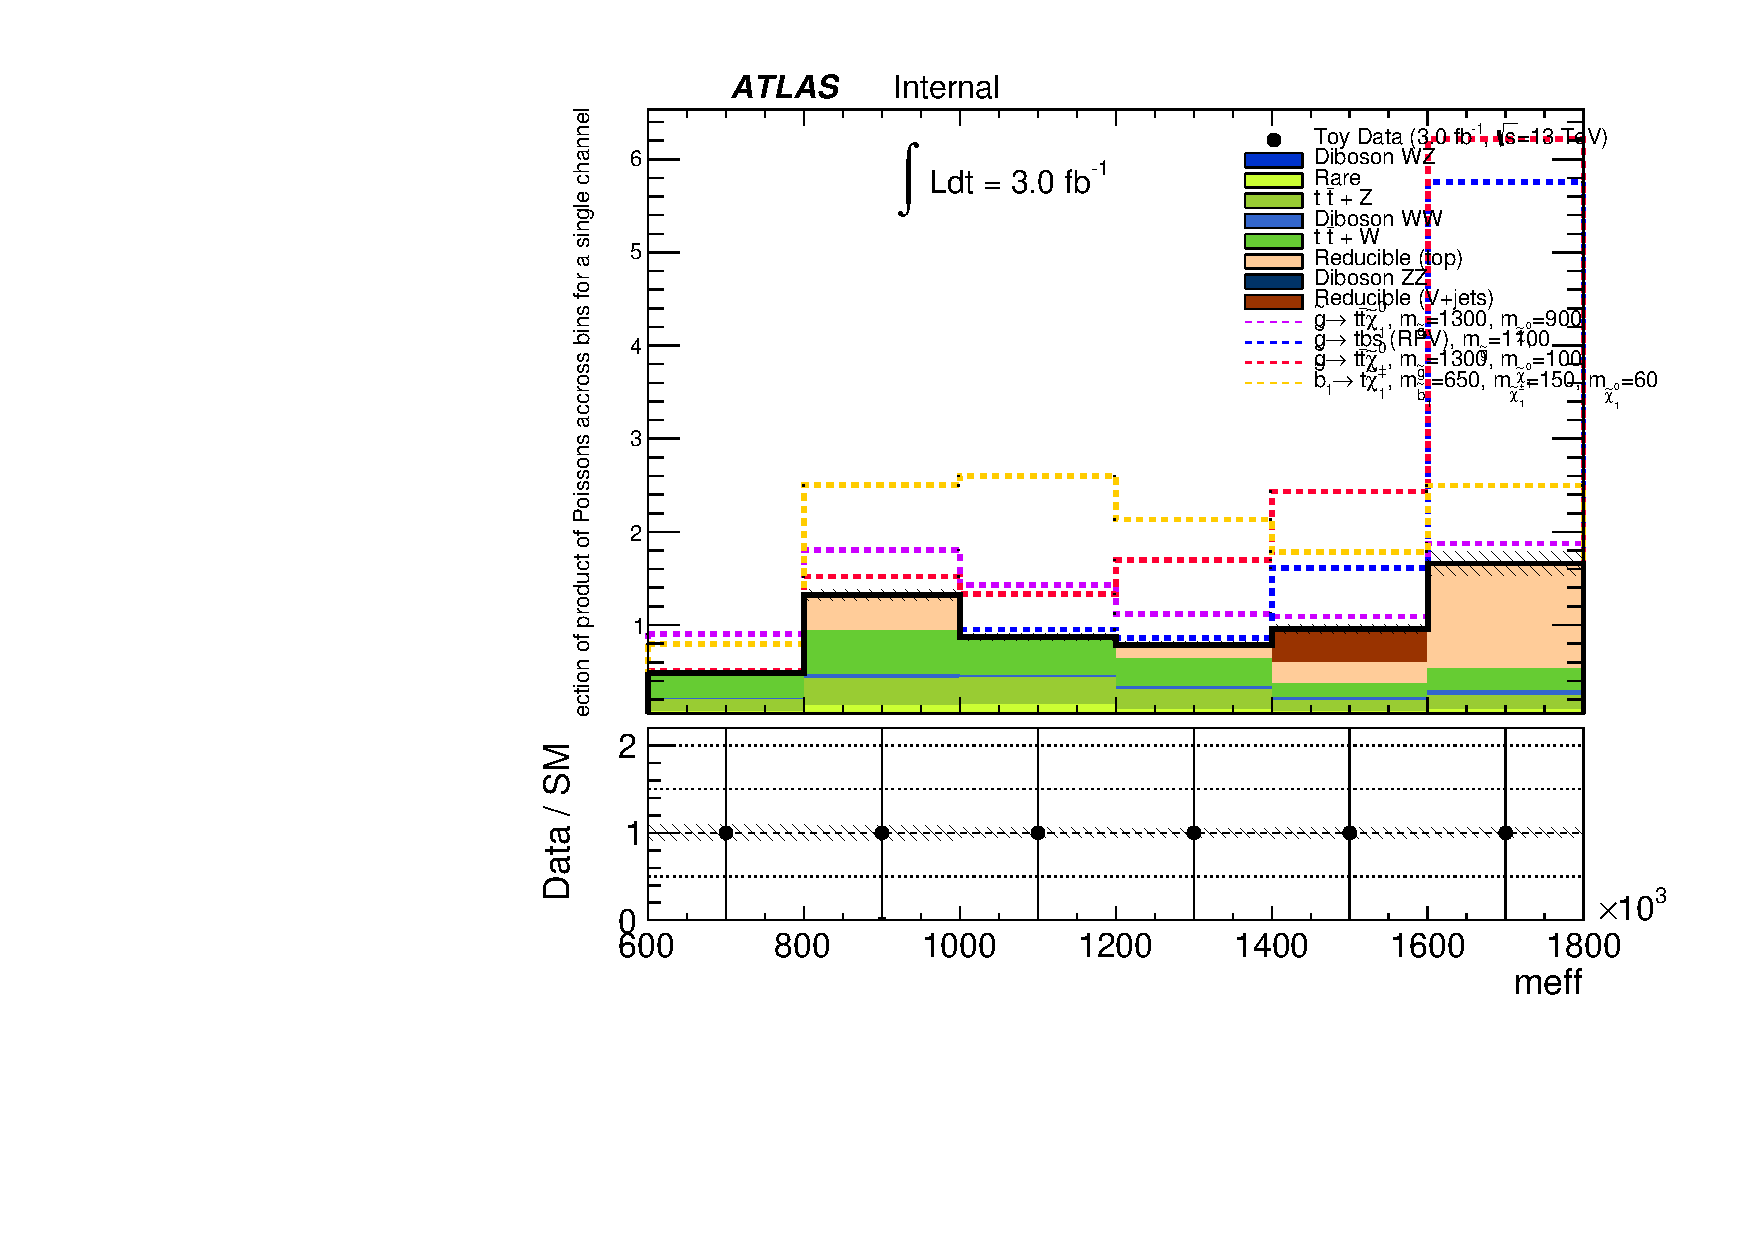
\includegraphics[width=0.49\textwidth]{HISTFITTER/can_SR1b150_binned_meff_beforeFit}}
\subfigure[$\met>100$, $\geq 4$ jets ($p_T>40$)]{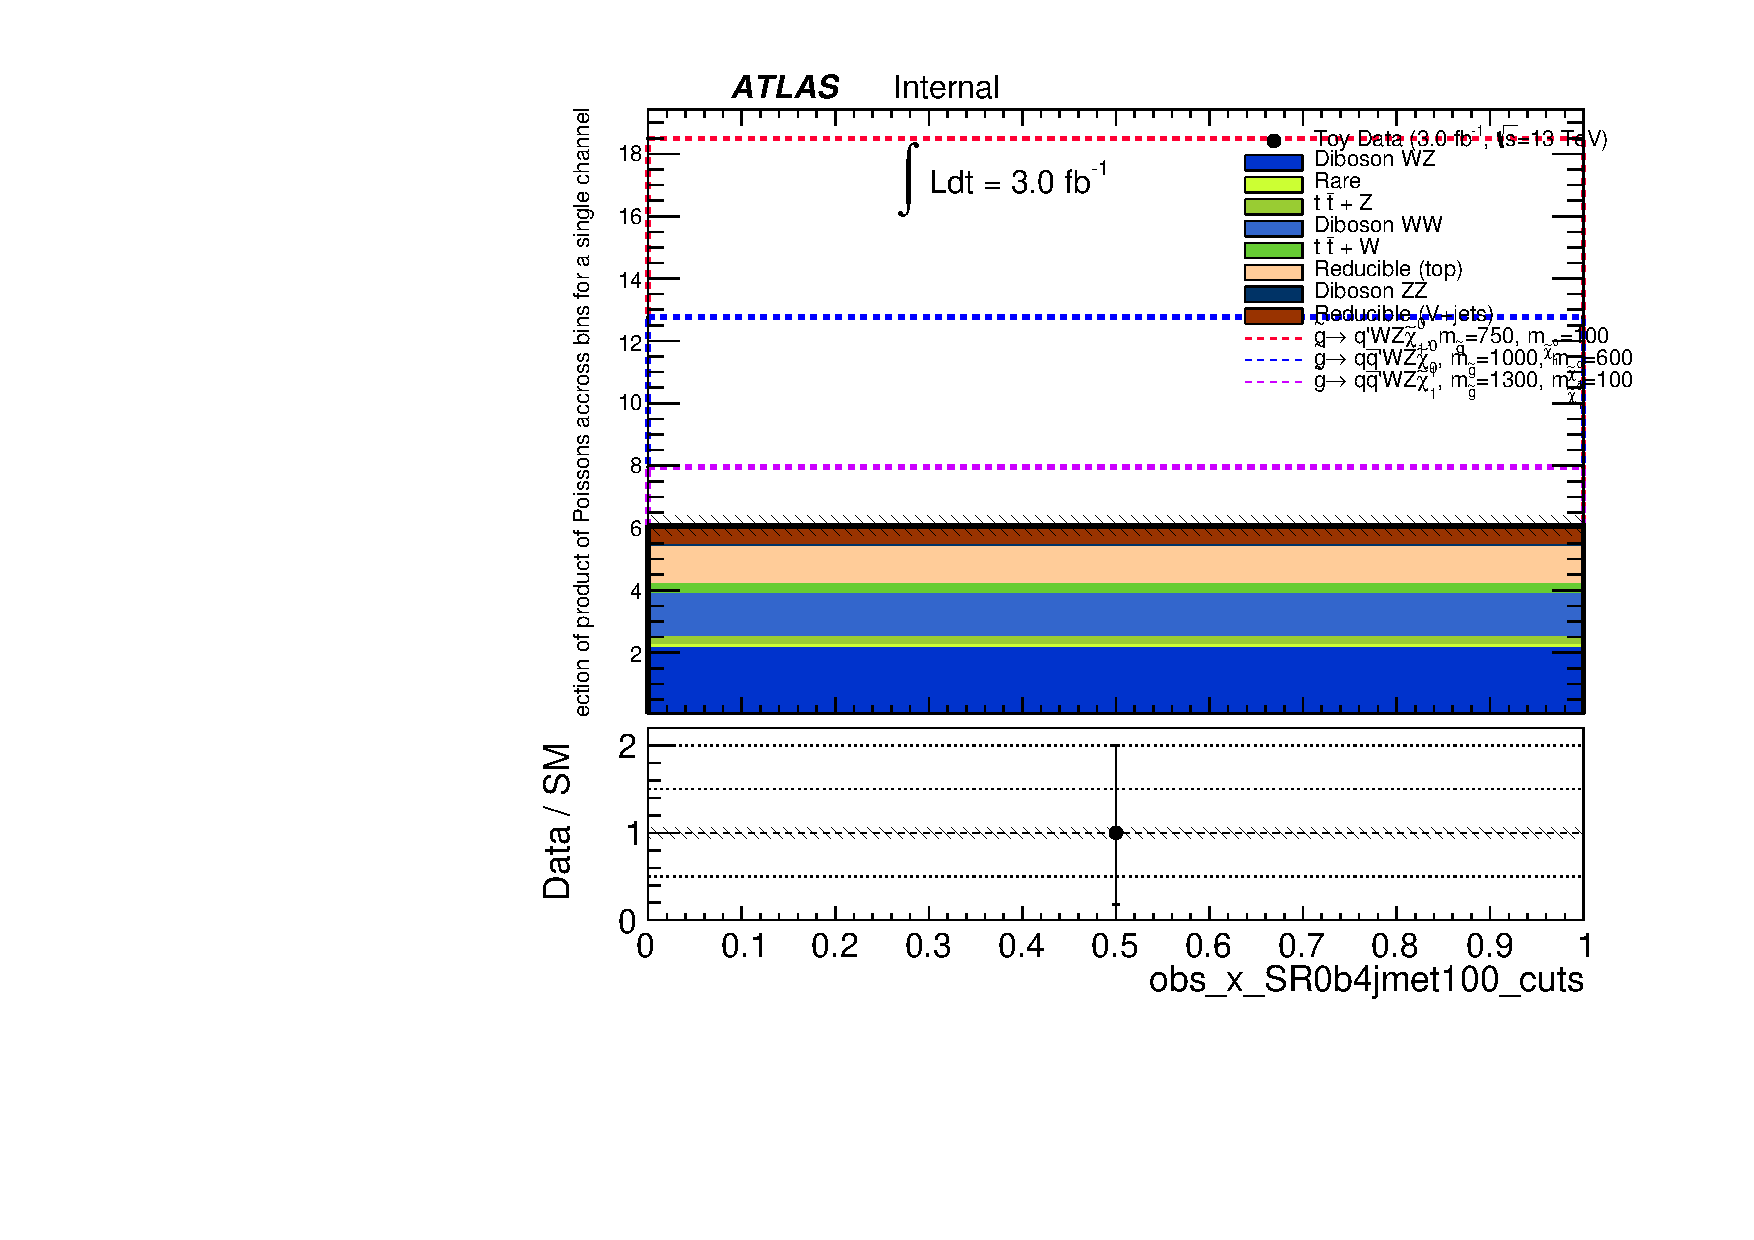
\includegraphics[width=0.49\textwidth]{HISTFITTER/can_SR0b4jmet100_cuts_beforeFit}}
\subfigure[$\met>200$, $\geq 4$ jets ($p_T>50$]{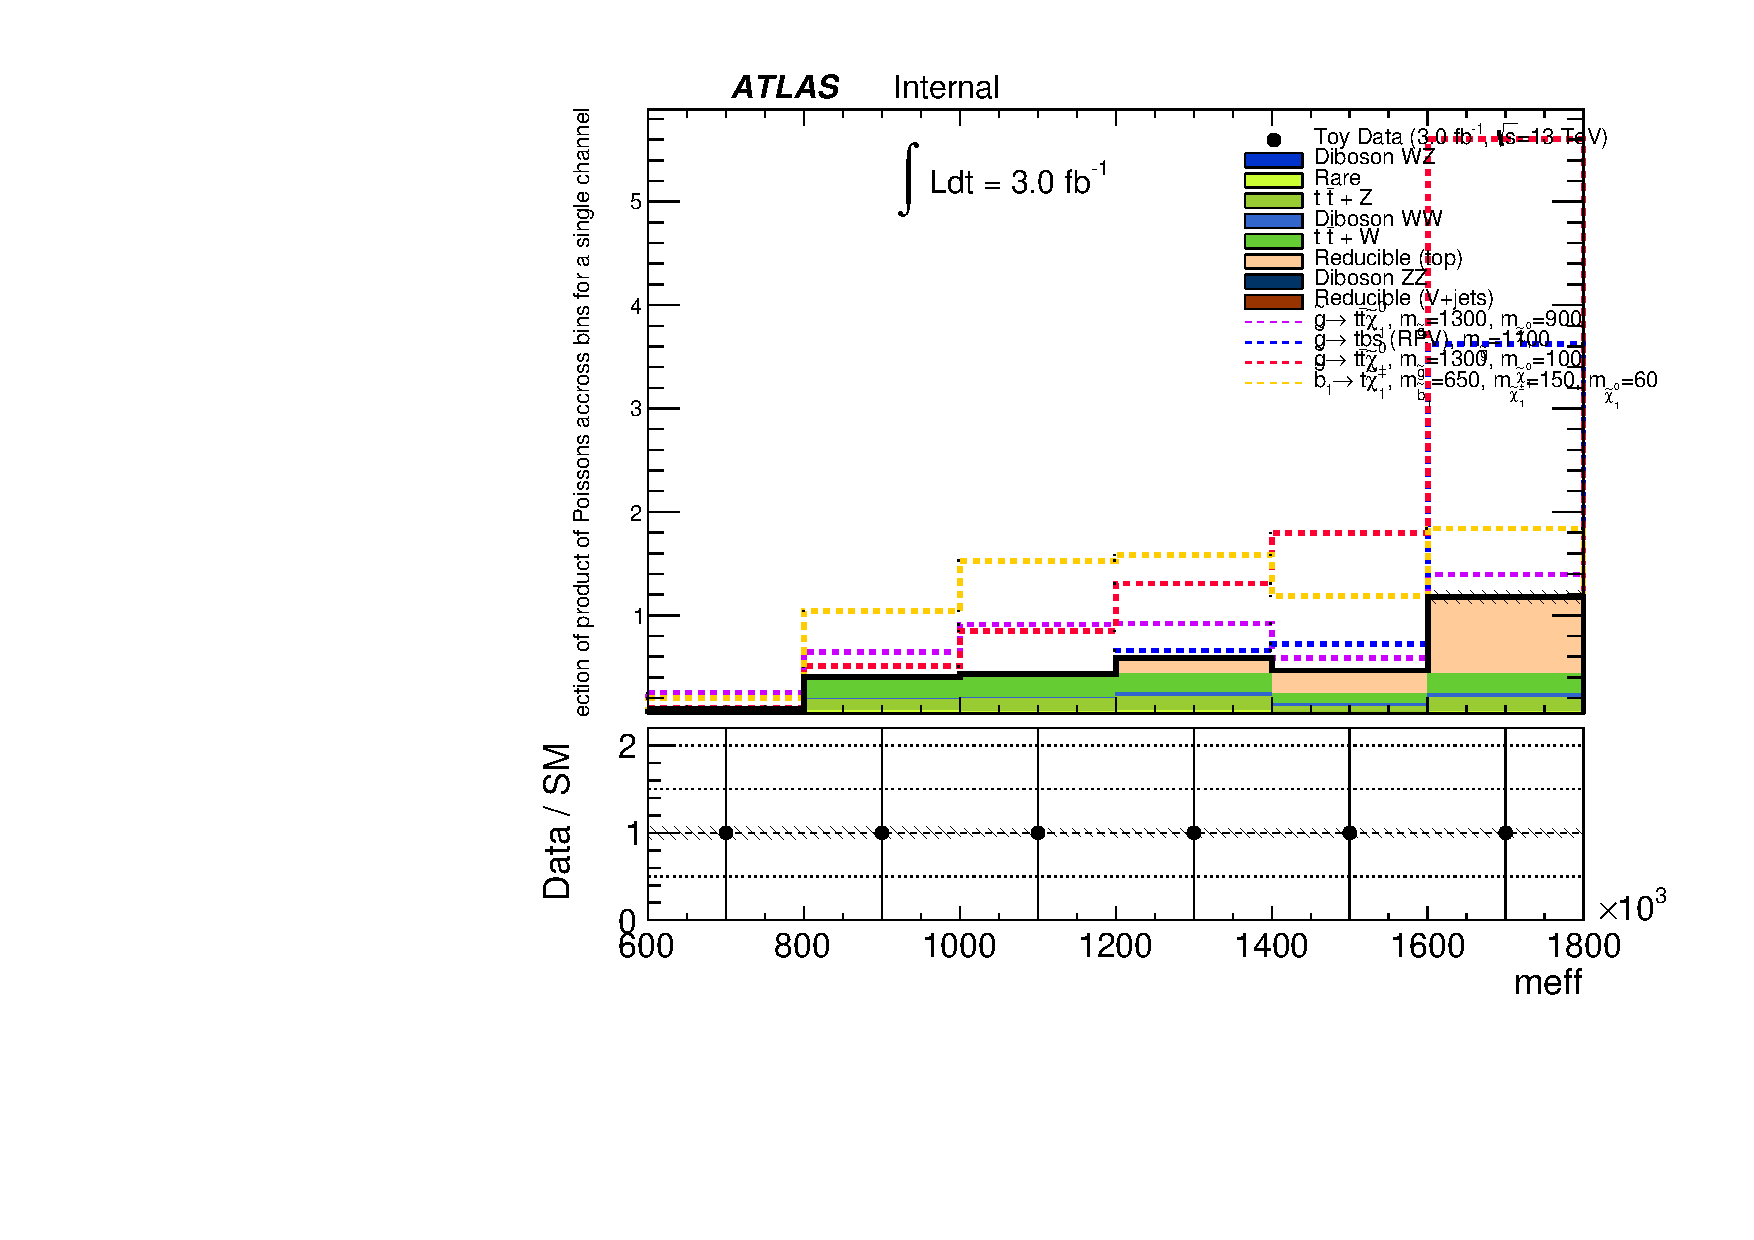
\includegraphics[width=0.49\textwidth]{HISTFITTER/can_SR1b200_binned_meff_beforeFit}}
\subfigure[$\met>100$, $\geq 5$ jets ($p_T>40$)]{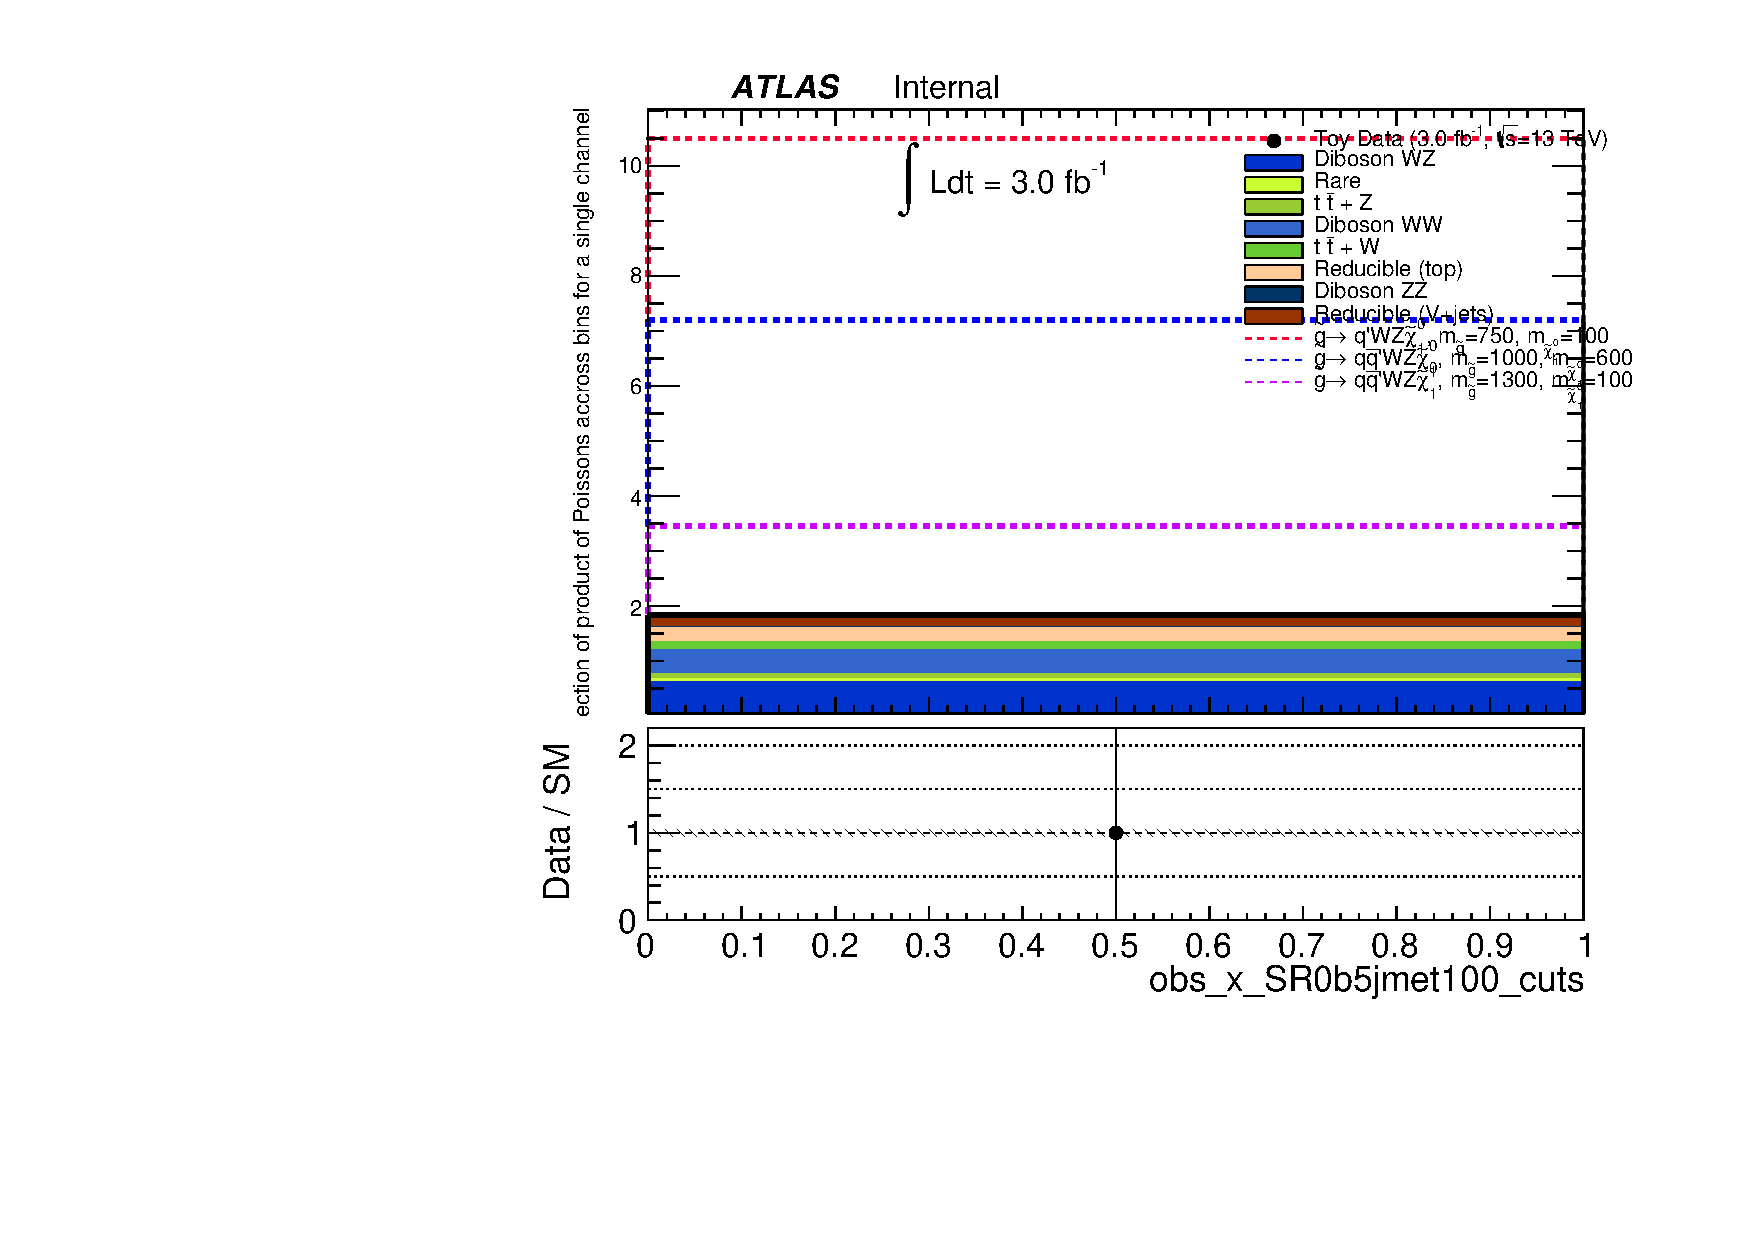
\includegraphics[width=0.49\textwidth]{HISTFITTER/can_SR0b5jmet100_cuts_beforeFit}}
\caption{Expected yields for Standard Model processes and a few characteristic signal scenarios, 
in selections with at least two same-sign leptons, at least one (left) or no $b$-jet (right), and the other cuts that define each of these signal region candidates. 
}
\label{fig:histfitter_sr0and1b}
\end{figure}


Figures~\ref{fig:histfitter_sr3b} and~\ref{fig:histfitter_sr0and1b} present the event yields of the background and a few characteristic signal scenarios, 
in various signal region candidates. The regions that have enough statistics to allow it are binned in the most relevant 
variable to discriminate between signal and background, either the effective mass or the number of jets (the latter for the 3 $b$-jets selection). 
Binnings are chosen such that the background yield in one bin remains at the level of around one event. 
One should note that they correspond to the binning used when performing shape fits as described in the next paragraph. 
\\
\par{\bf Sensitivity for the gluino stop offshell model\\}

\begin{figure}[htb!]
\centering
\subfigure{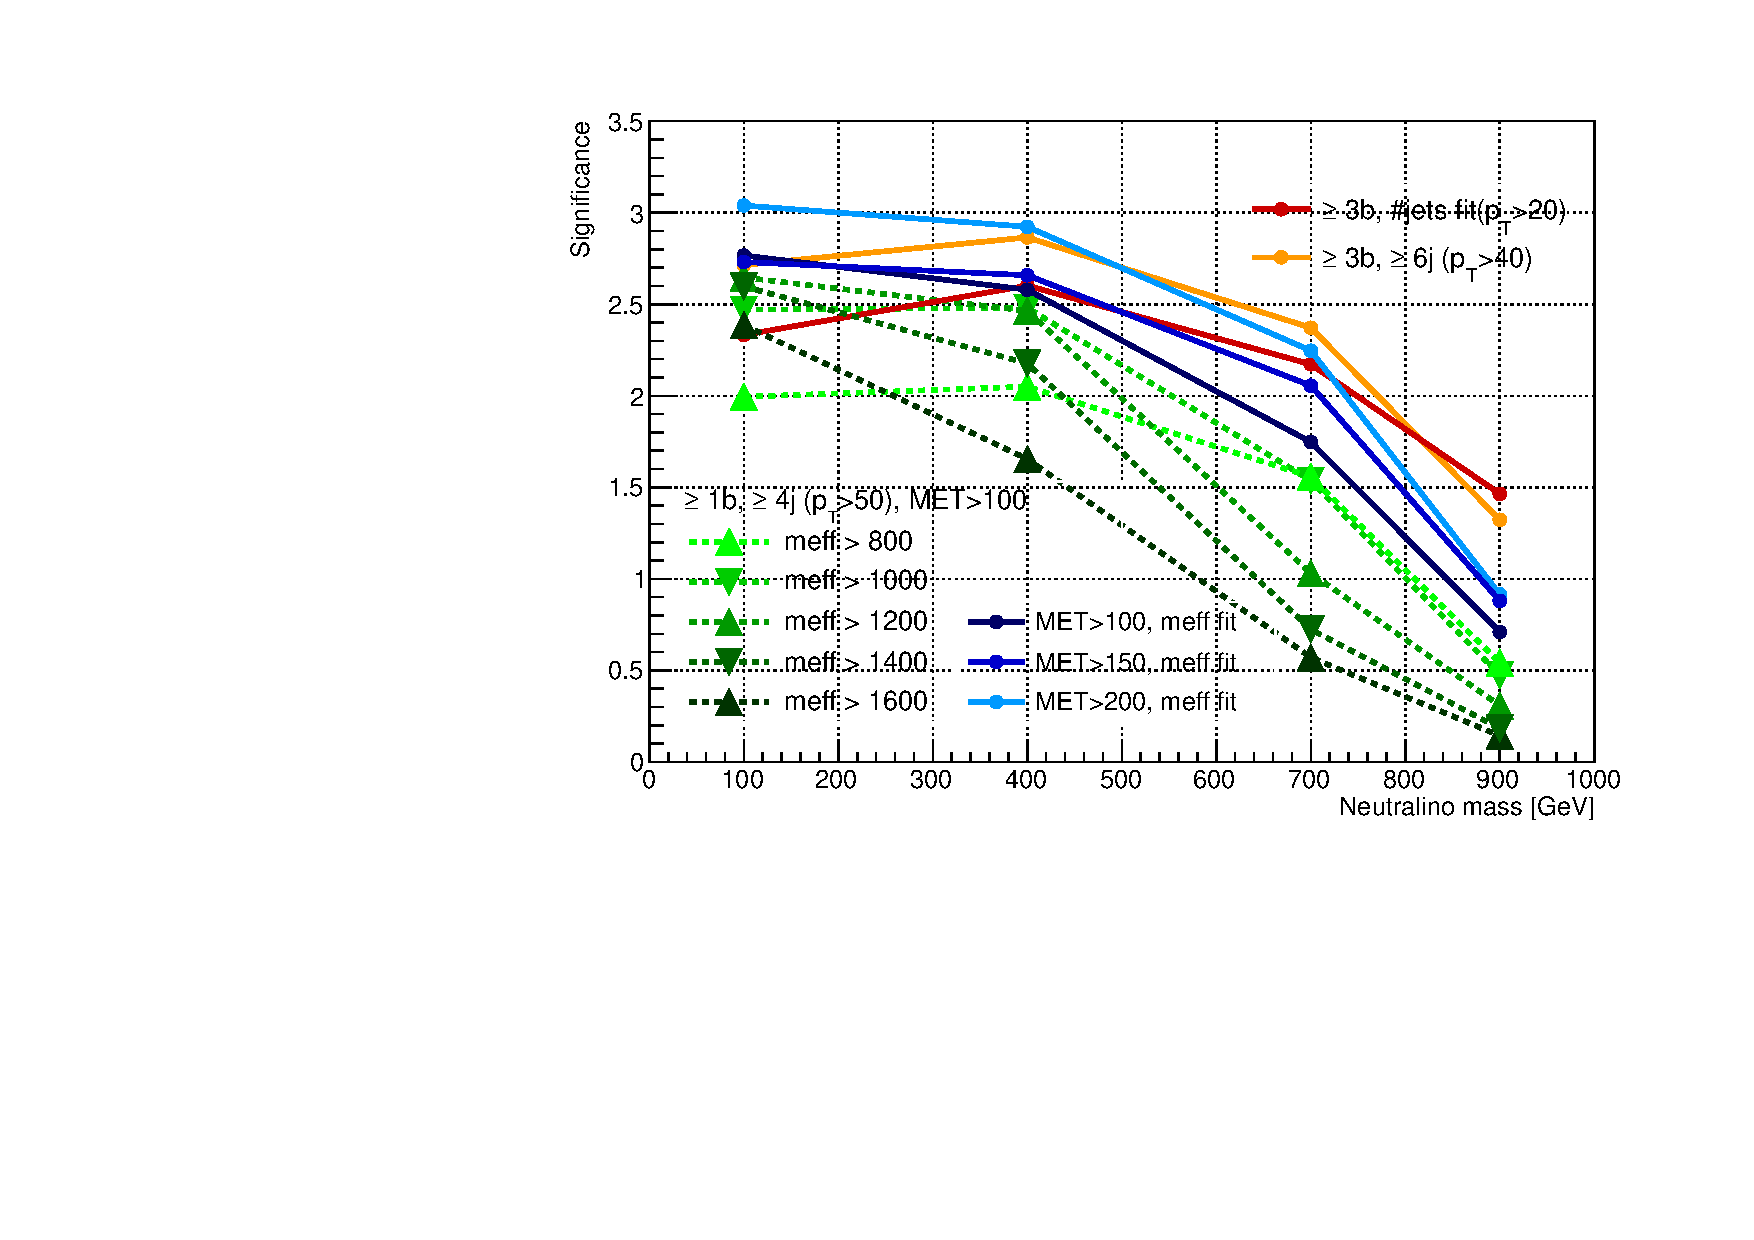
\includegraphics[width=0.49\textwidth]{HISTFITTER/gtt1300}}
\subfigure{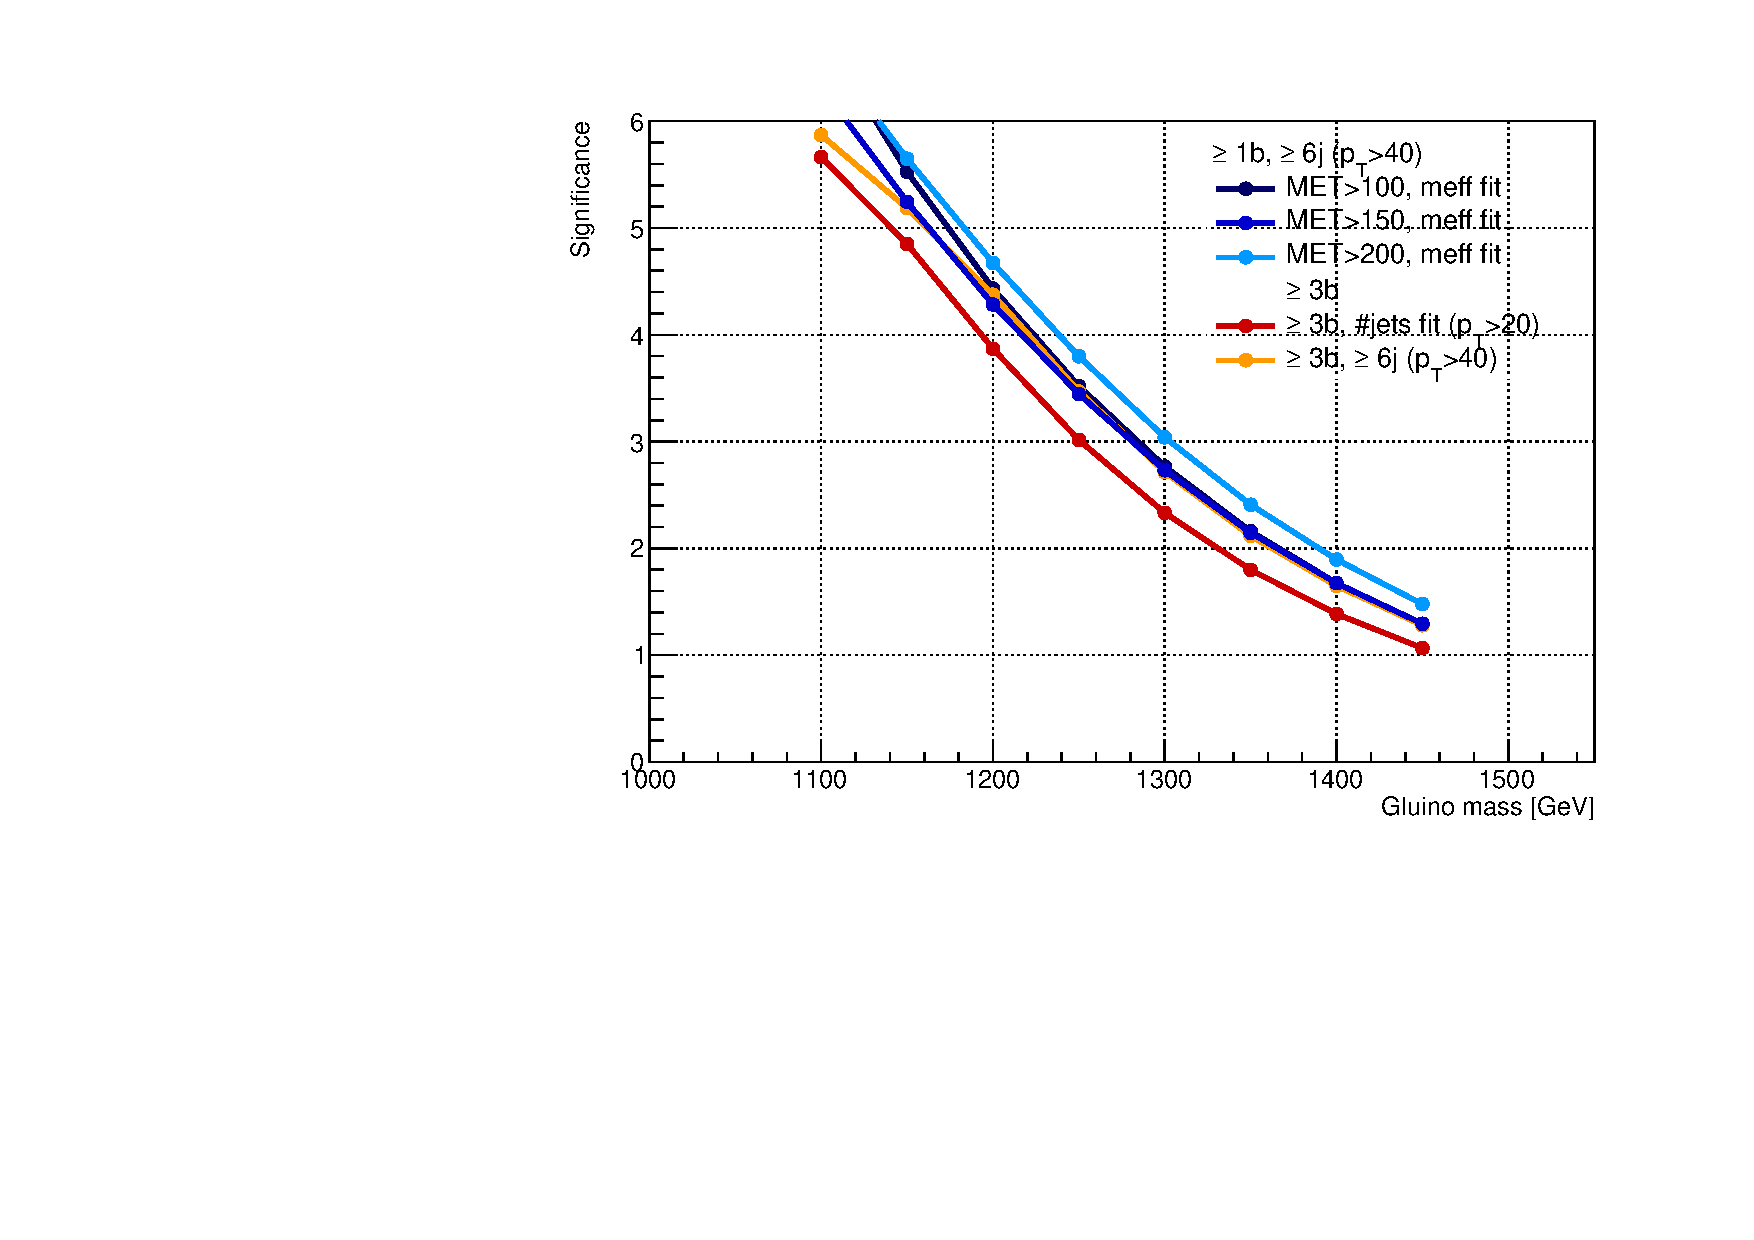
\includegraphics[width=0.49\textwidth]{HISTFITTER/gtt_lsp100}}
\caption{Expected signal significance for 3 fb$^{-1}$ for the gluino offshell stop model $\gluino\to t\bar{t}\neut$, 
varying the neutralino mass with a fixed gluino mass of 1300~\GeV (left) 
or extrapolating to different gluino masses from a reference point with gluino and neutralino masses of 1300 and 100~\GeV respectively (right). }
\label{fig:signif_gtt}
\end{figure}

\begin{figure}[htb!]
\centering
\subfigure{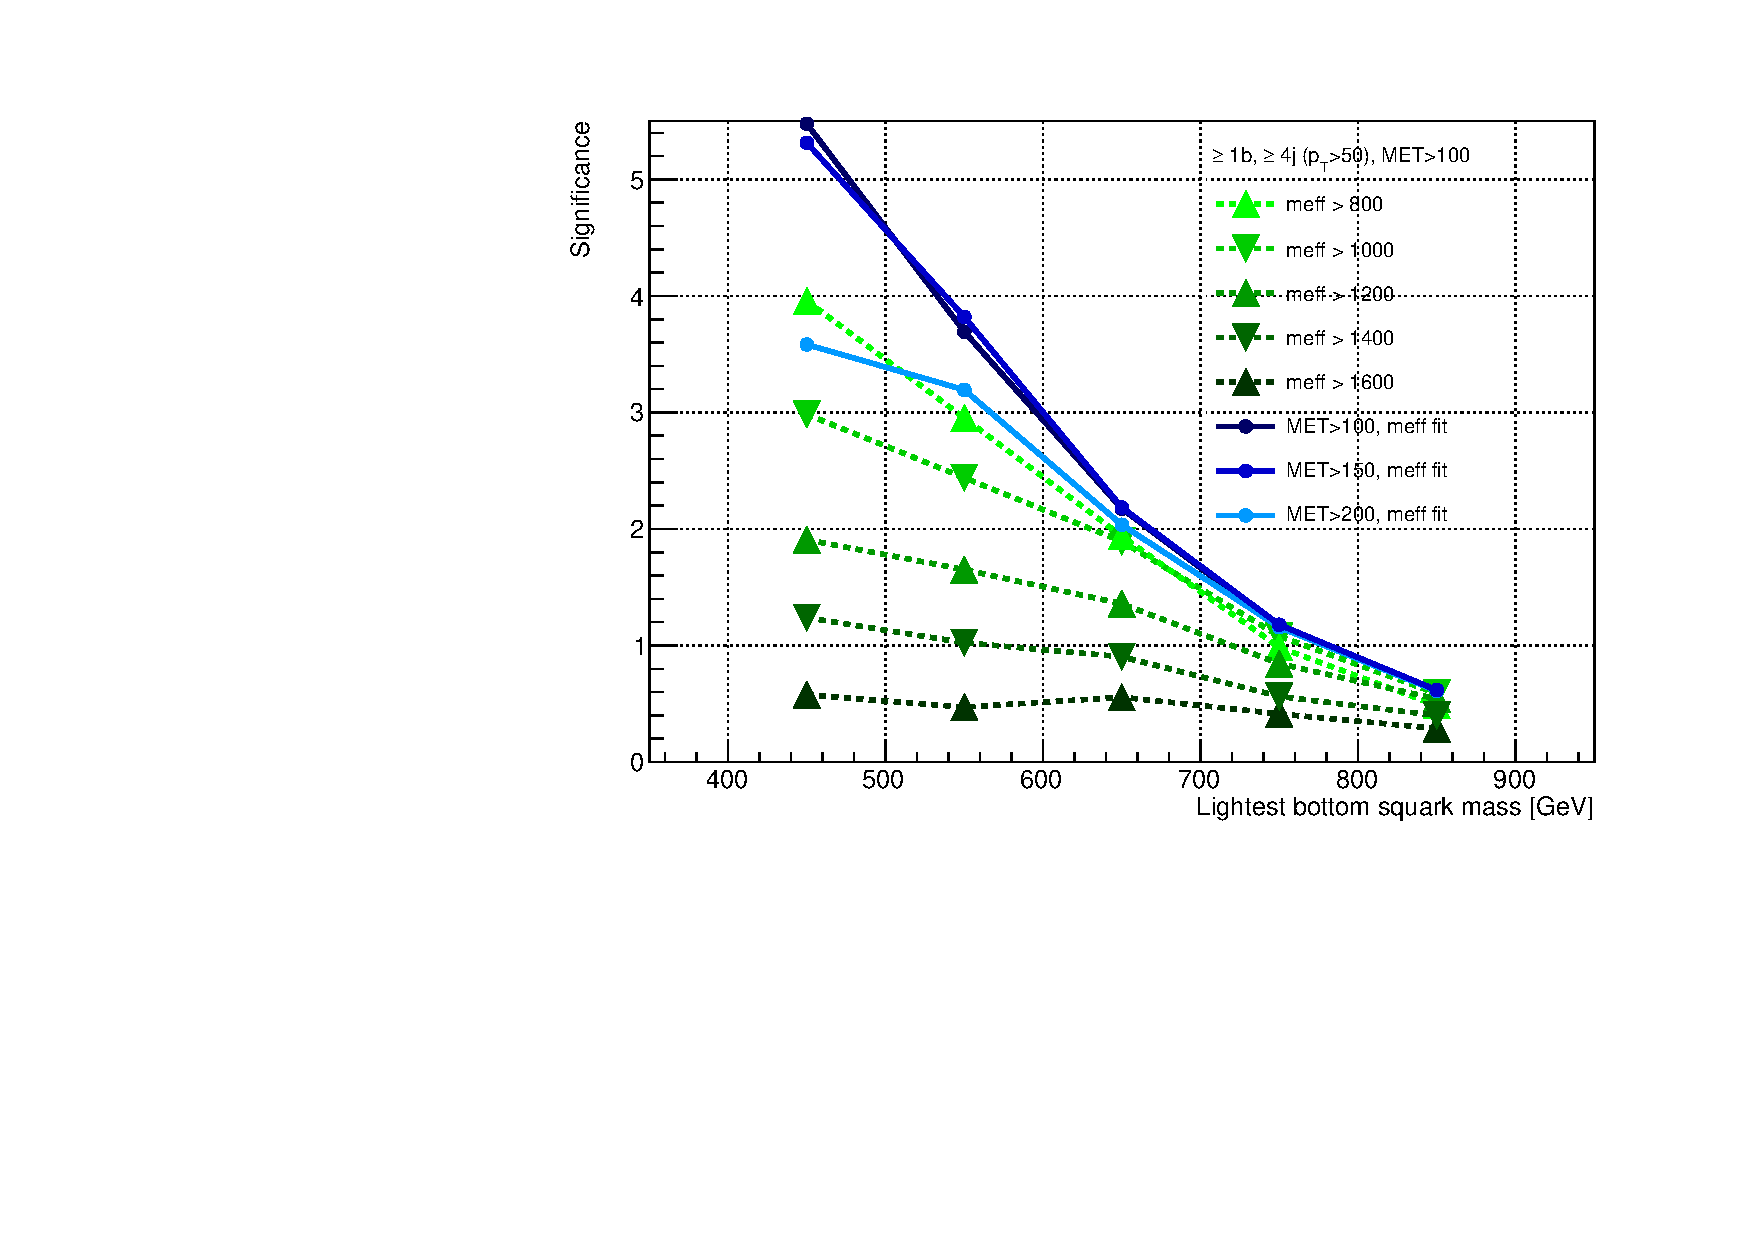
\includegraphics[width=0.49\textwidth]{HISTFITTER/sbottom}}
\subfigure{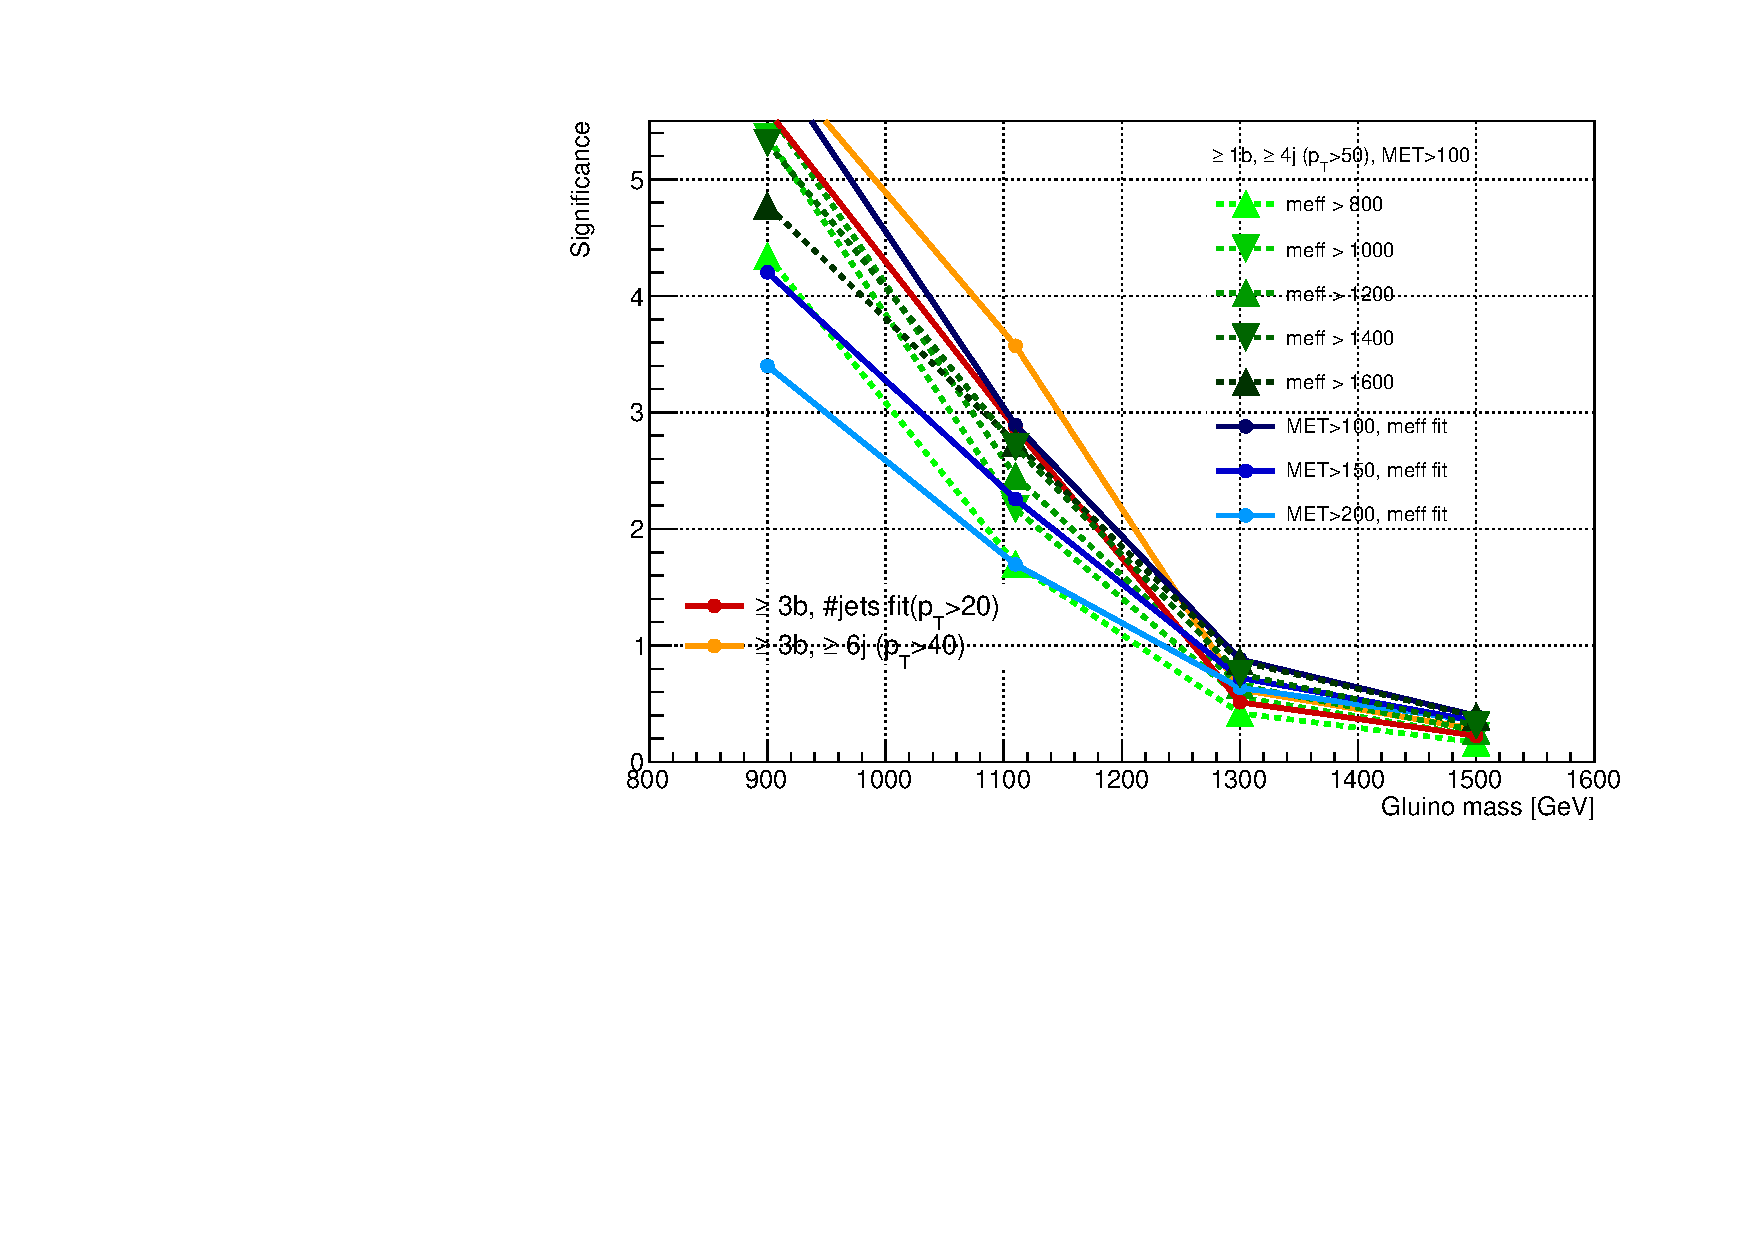
\includegraphics[width=0.49\textwidth]{HISTFITTER/rpv_tbs}}
\caption{Expected signal significance for 3 fb$^{-1}$ for the direct sbottom $\sbot\to t\chargino$ (left) 
or the gluino RPV $\gluino\to tbs$ (right) models. The neutralino mass is fixed to 100~\GeV in the sbottom scenario. }
\label{fig:signif_sbottom_and_rpv}
\end{figure}

\begin{figure}[htb!]
\centering
\subfigure{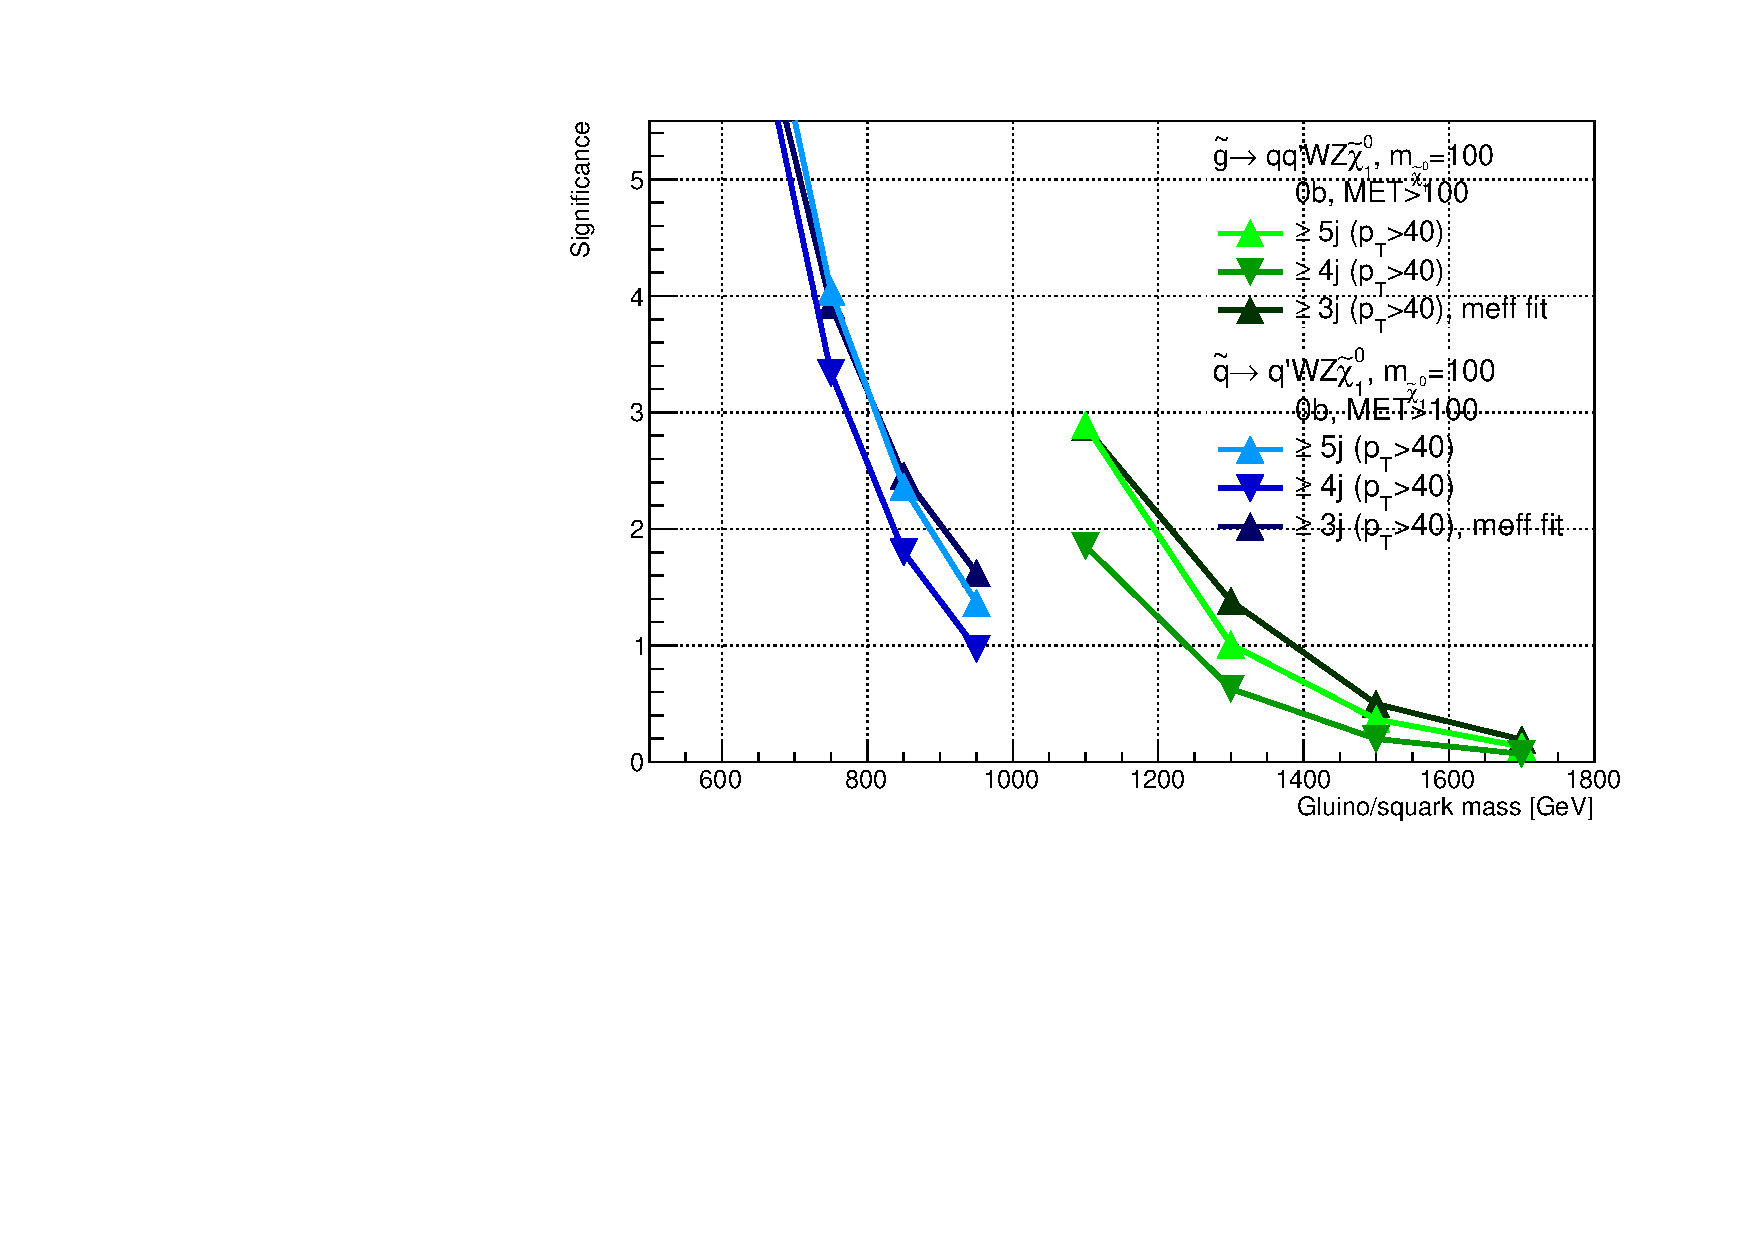
\includegraphics[width=0.49\textwidth]{HISTFITTER/firstgen_gq}}
\subfigure{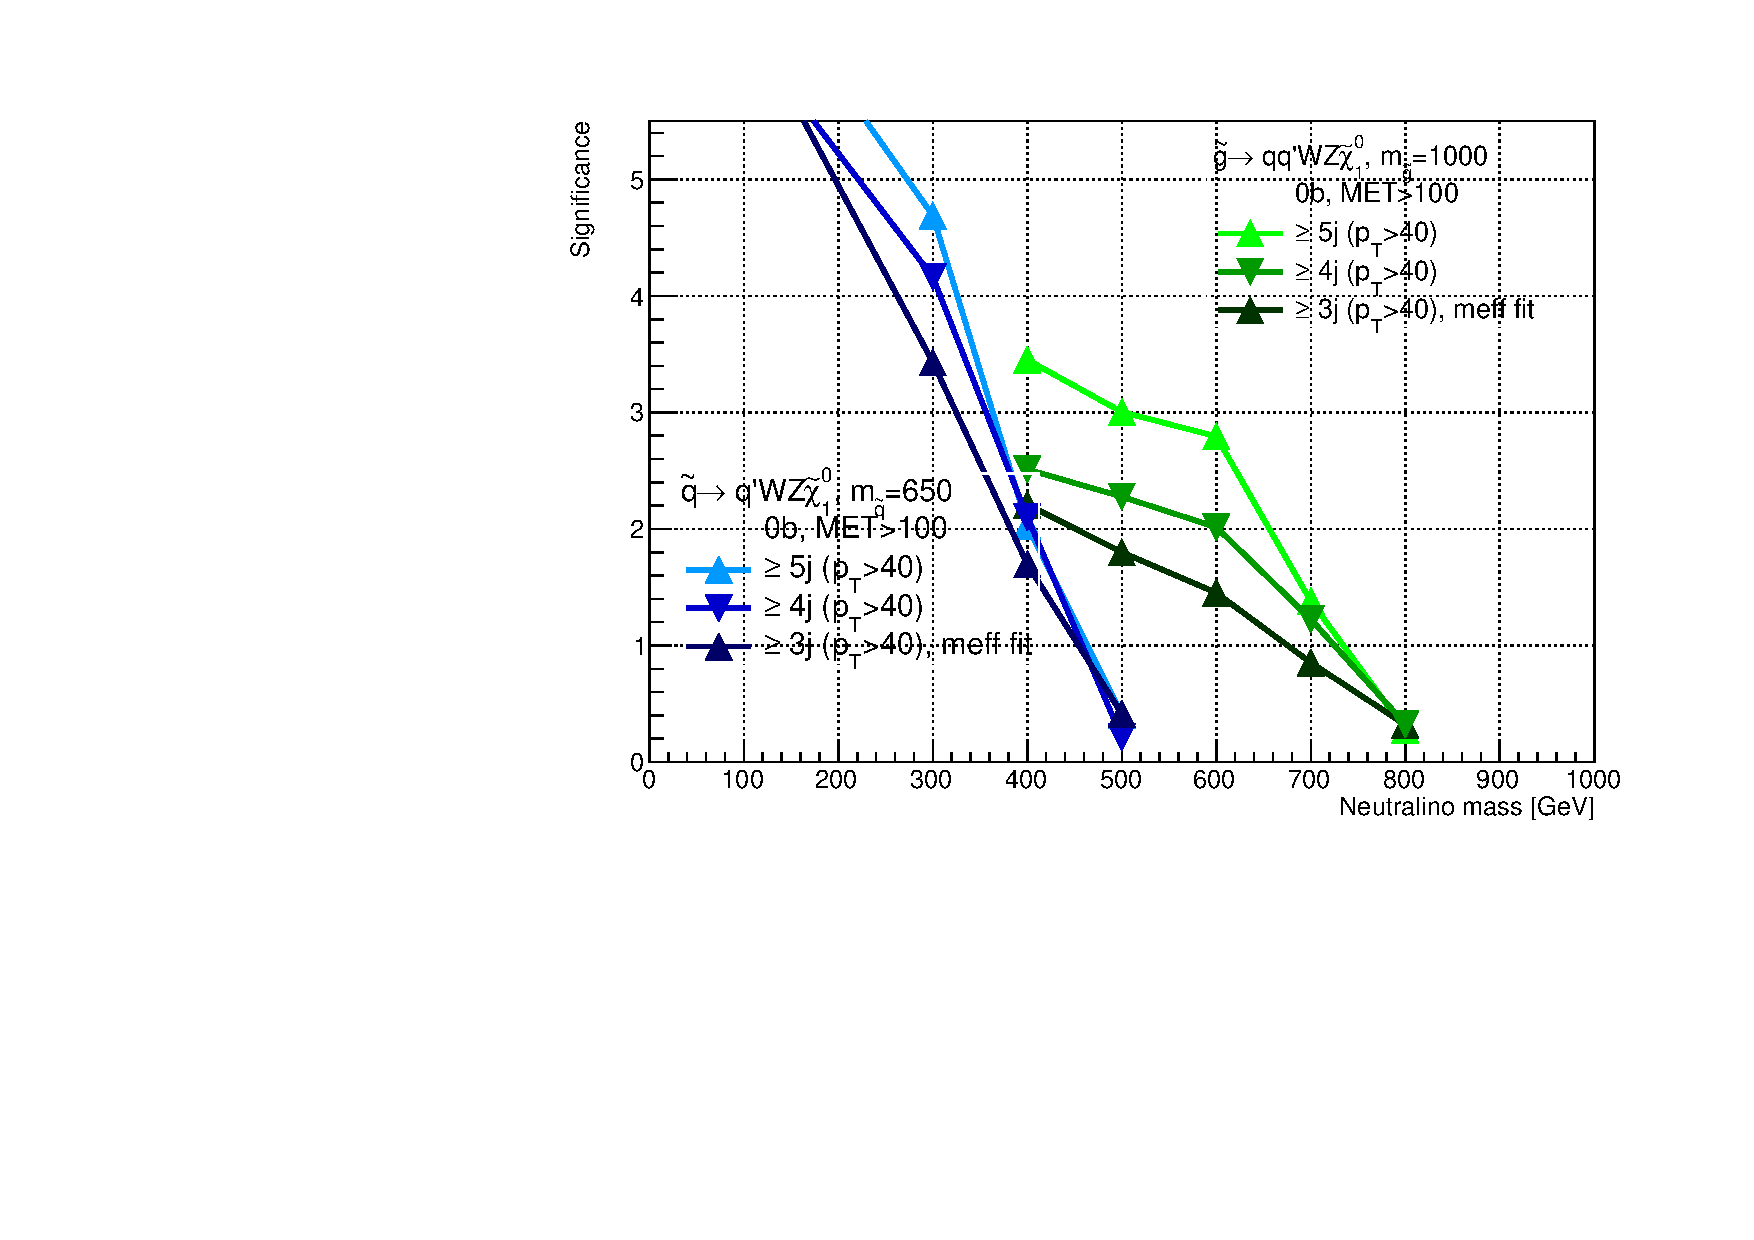
\includegraphics[width=0.49\textwidth]{HISTFITTER/firstgen_lsp}}
\caption{Expected signal significance for 3 fb$^{-1}$ for the gluino and squark 2-step decay models $\gluino/\tilde{q}\to q(q')WZ\neut$, 
varying the gluino or squark masses for a fixed neutralino mass of 100 GeV (left), 
or varying the neutralino mass for fixed gluino and squark masses of respectively 1000 and 650~\GeV. 
}
\label{fig:signif_firstgen}
\end{figure}

Figure~\ref{fig:signif_gtt} presents the signal significance obtained with several signal region candidates, for the gluino offshell stop model. 
For some of the regions, a shape fit of the effective mass or jet multiplicity distributions is performed. 
While it can provide additional benefit over simple cuts, the main reason for its use here was rather simply to avoid tuning cuts for each signal point. 
One can see indeed on the figure that for each mass, the significance obtained with an effective mass shape fit is rather close to the best 
of the significances computed with different choices of fixed cuts. 
As expected, at large neutralino mass signal regions based on $\geq 3$ $b$-jets perform better than the $\geq 1$ $b$-jet signal regions. 
There is not much difference in significance between the $\geq 3b$ selection requiring 6 hard jets and the one based on softer jets, 
possibly due to the fact that the mass spectra of the available grid points are not very compressed. 
One would probably see a larger difference for points lying on the diagonal $m_{\gluino}=2m_t+m_{\neut}$.

As only few signal samples have been generated, the projections 
Figure~\ref{fig:signif_gtt} (right) provides an estimate of the evolution of the sensitivity in a finer way, 
by simply using the kinematic distributions and yields obtained in a reference sample (gluino mass 1300~\GeV, neutralino mass 100~\GeV) 
weighted by the ratio of inclusive cross-sections between the mass to be extrapolated to, and the reference.  
It has been checked that the significance obtained from the next available sample (at a gluino mass of 1500~\GeV) matches rather closely the extrapolated value. 

One can conclude from these plots that at low neutralino mass and with such as low integrated luminosity, 
there is no sensitivity beyond the Run-1 exclusion. 
At higher neutralino mass however, the analysis would be sensitive to an area not yet excluded.  
\\
\par{\bf Sensitivity for the direct sbottom model\\}
Figure~\ref{fig:signif_sbottom_and_rpv} (left) shows the signal significance for several sbottom masses and a light neutralino. 
Here, the advantage of keeping a moderate $\met$ cut in the definition of the $\geq 1b$ signal region is clear. 
One can see that $2\sigma$ sensitivity up to masses of 650~\GeV might be expected, which is quite a nice improvement over the Run-1 reach 
(450~\GeV, although the expected limit was 50~\GeV higher). 
\\
\par{\bf Sensitivity for the gluino model with RPV stop decay\\}
The expected sensitivity for this model can be found on Fig.~\ref{fig:signif_sbottom_and_rpv} (right). 
The most powerful signal region for this model is as expected the selection with at least 3 $b$-jets and 6 hard jets. 
One can notice however that the signal regions with moderate $\met>100$~\GeV cut are quite sensitive as well : 
the absence of neutralinos is compensated by the presence of boosted tops decaying leptonically. 
\\
\par{\bf Sensitivity for the gluino and squark models with 2-step decays\\}
Finally, the performances of signal region definitions vetoing $b$-jets are probed with the gluino and squarks models with 2-step decays in gauge bosons. 
The signal significances for varied masses of gluino/squark or neutralino are provided on Fig~\ref{fig:signif_firstgen}. 
The signal region requiring 5 hard jets appears as the best compromise for both models, and in different regions of the phase space. 
For the gluino model, not much sensitivity beyong the Run-1 exclusion is gained at high gluino mass; 
at high neutralino mass, however, a significant non-excluded region up to neutralino masses of 650~\GeV seems to be at reach. 
For the squark model, on the other hand, one will be able to probe a new region of the phase space at high squark mass, up to 900~\GeV, which was not excluded in Run-1. 
